
La cinética del crecimiento bacteriano se encarga de estudiar el ritmo al que un cultivo dado de células crece a lo largo del tiempo.

Este ritmo de crecimiento puede variar en base a varios factores. Algunos de ellos pueden ser:

\begin{itemize}
    \item El tipo de sustrato y su disponibilidad.
    \item Las condiciones fisicoquímicas del ambiente (temperatura y pH, principalmente.).
    \item El tamaño de la población en el medio.
    \item Presencia de sustancias que aceleren o ralentizen el crecimiento bacteriano.
\end{itemize} 

\section{Curvas de crecimiento bacteriano}

El crecimiento típico de un microorganismo se describe en la conocida curva de crecimiento bacteriano, cuya ejemplificación podemos observar en la \autoref{fig:curva_crecimiento_bacteriano}. Esta se compone de las siguientes fases:

\begin{enumerate}
    \item Fase de latencia o lag: Las velocidades de reproducción y de muerte son iguales. Consta de una adaptación al medio. Se activan principalmente mecanismos de mantenimiento celular.
    \item Fase logarítmica o log: La velocidad de reproducción es mayor a la de muerte, por ende, hay un crecimiento rápido. Predomina la producción de metabolitos primarios.
    \item Fase estacionaria: Las velocidades de reproducción y de muerte son de nuevo iguales. Predomina la producción de metabolitos secundarios.
    \item Fase de muerte: Aquí la velocidad de muerte es ahora mayor a la de reproducción.
\end{enumerate}

\begin{figure}[H]
    \centering
    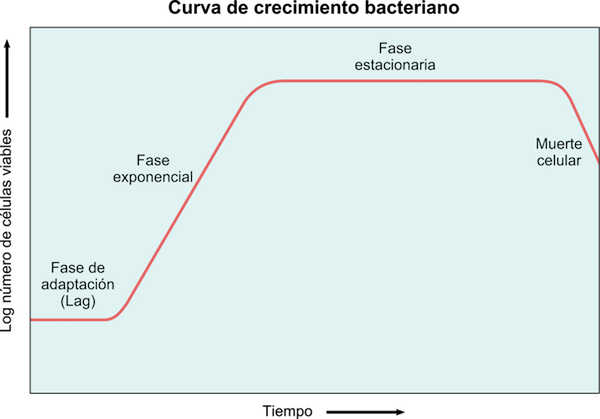
\includegraphics[width=0.6\linewidth]{07_curva_de_crecimiento_bacteriano}
    \caption{Ejemplo de curva de crecimiento bacteriano}
    \label{fig:curva_crecimiento_bacteriano}
\end{figure}

En medios con múltiples sustratos, algunos microorganismos pueden mostrar múltiples fases logarítmicas, cada una con una fase estacionaria intermedia, en la cual el microorganismo realiza una serie de adaptaciones en su maquinaria enzimática para así poder degradar el nuevo sustrato. Un ejemplo de esto se muestra en la \autoref{fig:curva_diauxica}.

\begin{figure}[H]
    \centering
    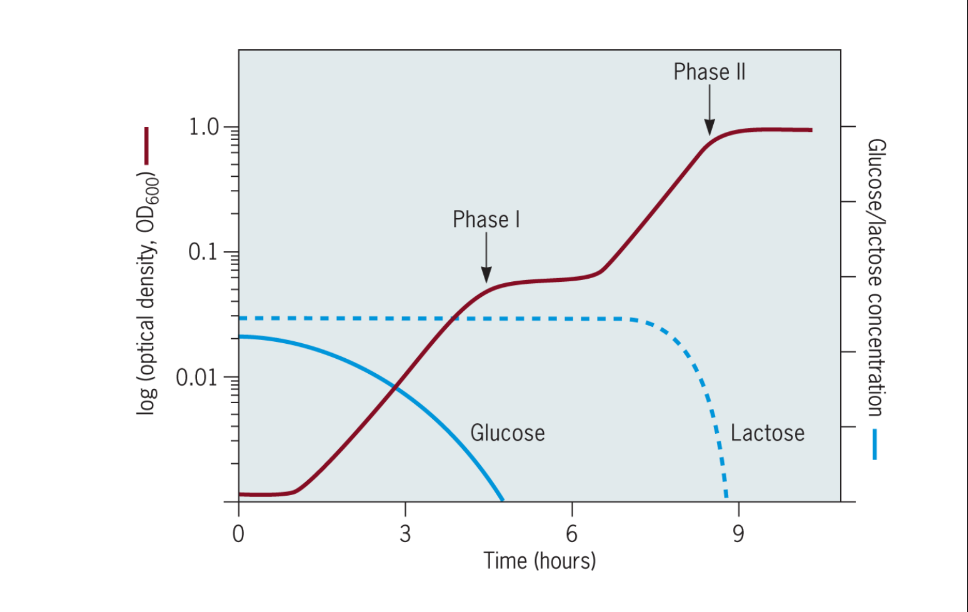
\includegraphics[width=0.8\linewidth]{07_curva_diauxica}
    \caption[Ejemplo de curva diáuxica]{Ejemplo de curva diáuxica. Se observa una correspondencia entre el consumo de glucosa y la primer fase log, así como del consumo de lactosa y la segunda fase log, así como una fase estacionaria intermedia, esto en el proceso para adaptar la maquinaria enzimática del microorganismo para poder degradar lactosa.}
    \label{fig:curva_diauxica}
\end{figure}

\section{Crecimiento exponencial de microorganismos}

Todas estas curvas son al final del día una representación gráfica del ritmo a la que los microorganismos se reproducen. Tal reproducción sigue un ritmo exponencial, esto porque los microorganismos al reproducirse parten de una célula para producir dos.\footnote{Así es para muchos microorganismos, más no para todos. Aún así, en bioprocesos se suele trabajar con microorganismos que siguen el típico crecimiento de fisión binaria.}. Vease por ejemplo la \autoref{fig:crecimiento_exponencial}.

Así pues, el crecimiento se puede representar con $2^{n}$, siendo $n$ el número de divisiones o generaciones que han transcurrido.

\begin{figure}[H]   
    \centering
    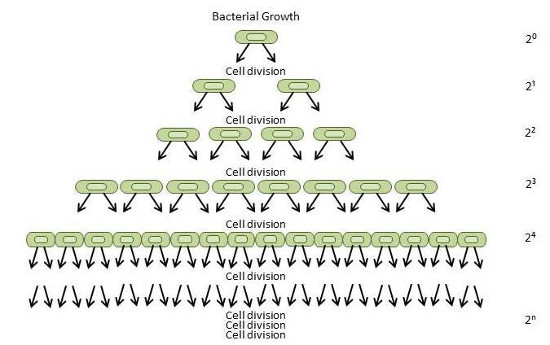
\includegraphics[width=0.6\linewidth]{07_crecimiento_exponencial}
    \caption[Representación gráfica del crecimiento exponencial bacteriano]{Representación gráfica del crecimiento exponencial bacteriano. Se puede apreciar el aumento del exponente de $2^{n}$ con cada división}
    \label{fig:crecimiento_exponencial}
\end{figure}

Tomando esto encuenta, podemos calcular la población en la que un cultivo de microorganismos se encuentra de la siguiente manera:

\begin{equation}\label{eq:nt}
    N_{t} = N_{0} \cdot 2^{n}
\end{equation}

Siendo $N_{0}$ la población con la que se inició, o población inicial, y $N_{t}$ la población actual del cultivo despues de pasadas las $n$ generaciones especificadas en $2^{n}$. 

Ahora, estos datos pueden graficarse de manera directa y se obtendría una linea exponencial sin embargo, puede resultar mejor aplicarles un logaritmo para obtener una linea recta, que puede ser estudiada con la respectiva ecuación de la recta ($y=mx+b$). Las diferencias entre ambas formas de graficar el crecimiento se muestran en la \autoref{fig:crecimiento_bacteriano_log}.

\begin{figure}[H]
    \centering
    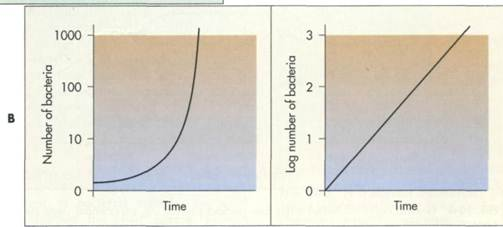
\includegraphics[width=0.8\linewidth]{07_crecimiento_bacteriano_log}
    \caption{Diferencia entre gráfica con número directo de bacterias y gráfica con escala logarítmica}
    \label{fig:crecimiento_bacteriano_log}
\end{figure}

\section{Tiempo de duplicación ($t_{d}$)}

Tal vez un elemento más importante en bioprocesos sea el tiempo de duplicación o generación, que se representa como $t_{d}$. Este representa el tiempo que un microorganismo necesita para duplicarse, y nos aporta información sobre qué tan rápido un cultivo crecerá. Se prefieren entonces tiempos de duplicación lo más bajos posibles cuando se trata de laproducción de biomasa o de la obtención de algún subproducto. Este valor se ve afectado por las condiciones del medio (sustrato, temperatura, pH, etcétera).

Para calcular el tiempo de duplicación de un microorganismo dado solo necesitamos el siguiente cálculo:

\begin{equation}
    t_{d} = \frac{t}{n}
\end{equation}

Siendo $t$ el tiempo que ha transcurrido y $n$ el número de generaciones que han transcurrido.

\section{Generaciones transcurridas ($n$)}

Ahora, en caso de no contar con el número de generaciones transcurridas podemos despejar la \autoref{eq:nt}:

\begin{align*}
    N_{t} = N_{0} \cdot 2^{n} \quad \longrightarrow \quad \log(N_{t}) = \log(N_{0}) - n \cdot \log(2) \quad \longrightarrow \quad \frac{\log(N_{t}) - \log(N_{0})}{\log(2)} = n
\end{align*}

Para obtener así:

\begin{equation}\label{eq:n}
    n = \frac{\log(N_{t}) - \log(N_{0})}{\log(2)}
\end{equation}

Es con esta ecuación que podemos obtener la generaciones que han pasado en un cultivo, unicamente haciendo uso de la población inicial y la población final.

\section{Cinética ($\mu$)}

Dado que la cinética estudia el cambio, a la cinética de crecimiento bacteriano le interesa saber el ritmo a la que un cultivo dado crece en distintos puntos del tiempo. El cambio en la cantidad de biomasa puede representarse con la siguiente ecuación:

\begin{equation*}
    r_{x} = \mu x
\end{equation*}

Esto también podemos expresarlo como una ecuación diferencial de la siguiente manera:

\begin{equation}\label{eq:ux}
    \frac{dx}{dt} = \mu x
\end{equation}

Esta nos dice cuanto cambia la cantidad de biomasa ($x$) respecto al tiempo ($t$). A su vez, $\mu$ es la velocidad específica a la que se da ese crecimiento bacteriano.

Para calcular $\mu$ solo necesitamos resolver la ecuación diferencial de la \autoref{eq:ux}, esto de la siguiente manera:

\begin{align*}
    \frac{dx}{dt} = \mu x & \longrightarrow \frac{1}{x} \ dx = \mu \ dt
    \\
    \\
    \int_{x_{0}}^{x}{\frac{1}{x}} \ dx = \int_{t_{0}}^{t_{d}}{\mu \ dt} &\longrightarrow \ln(x) - \ln(x_{0}) = \mu \cdot (t_{d} - 0)
\end{align*}

Despenjando tendríamos:

\begin{equation}
    \mu = \frac{\ln(x) - \ln(x_{0})}{t}
\end{equation}

Es con esta ecuación que podemos calcular $\mu$ unicamente haciendo uso de de las poblaciones de un cultivo dado ($x$ y $x_{0}$) y el tiempo transcurrido ($t$), y así saber a qué velocidad se está reproduciendo un microorganismo en un momento dado.